\documentclass[ignorenonframetext,8pt,aspectratio=169]{beamer}
\usepackage{umut}
\usepackage{umuttr}
\usepackage{usynsem}
\usepackage[utf8]{inputenc}
\usepackage{uling}
\usepackage{natbib,unatbib}
\usepackage{linguex}
         \renewcommand{\refdash}{}
\usepackage{ubeamer}
\usepackage{verbatim}
\usepackage{adjustbox}
\usepackage{fancyvrb}

\usepackage{ulem}

\usepackage{tikz-qtree}
\usetikzlibrary{er,positioning}

\title{Layered VPs}
\author{\  \\  {\it Based on Koeneman \& Zeiljstra (2017)} \\ \vspace{20pt} Umut \"Ozge\\  }

\date{COGS 532: Theoretical Linguistics\\ METU, Informatics}

\begin{document}

\begin{frame}\frametitle{}
\thispagestyle{empty}
\maketitle
\end{frame}

\begin{frame}[t,plain]{Structure of ditransitives}

\ex. They give Mary flowers.

\vspace{20pt}
\hspace{60pt}
\adjustbox{valign=t}{
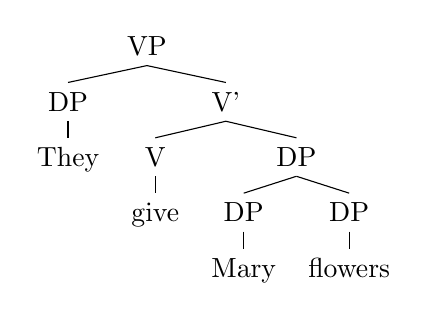
\begin{tikzpicture}
\tikzset{level distance=20pt, sibling distance=5pt}
\tikzset{every tree node/.style={align=center,anchor=north}}

\Tree[.{VP} [.{DP} They ] [.{V'} [.{V} give ] [.{DP} [.{DP} Mary ] [.{DP} flowers ] ] ] ] 

\end{tikzpicture}}
\hspace{60pt}
\adjustbox{valign=t}{
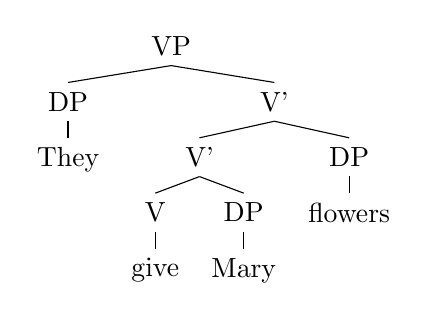
\begin{tikzpicture}
\tikzset{level distance=20pt, sibling distance=5pt}
\tikzset{every tree node/.style={align=center,anchor=north}}

\Tree[.{VP} [.{DP} They ] [.{V'} [.{V'} [.{V} give ] [.{DP} Mary ] ] [.{DP} flowers ] ] ] 

\end{tikzpicture}}


\end{frame}

\begin{frame}[t,plain]{Argument from case}

\ex. They give Mary flowers.

\vspace{20pt}
\hspace{60pt}
\adjustbox{valign=t}{
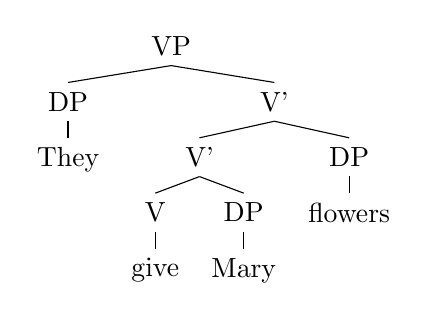
\begin{tikzpicture}
\tikzset{level distance=20pt, sibling distance=5pt}
\tikzset{every tree node/.style={align=center,anchor=north}}

\Tree[.{VP} [.{DP} They ] [.{V'} [.{V'} [.{V} give ] [.{DP} Mary ] ] [.{DP} flowers ] ] ] 

\end{tikzpicture}}
\end{frame}

\begin{frame}[t,plain]{Argument from binding}

\ex. \a. John showed Mary\ind{i} herself\ind{i}.
\b. The teacher gave [every girl]\ind{i} her\ind{i} favorite toy.

\vspace{20pt}
\hspace{60pt}
\adjustbox{valign=t}{
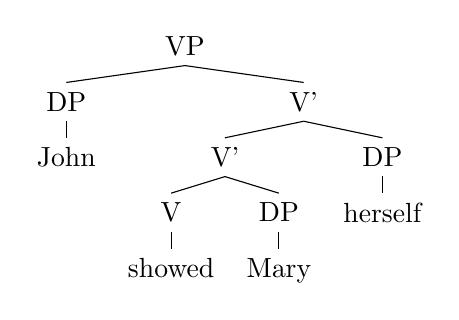
\begin{tikzpicture}
\tikzset{level distance=20pt, sibling distance=5pt}
\tikzset{every tree node/.style={align=center,anchor=north}}

\Tree[.{VP} [.{DP} John ] [.{V'} [.{V'} [.{V} showed ] [.{DP} Mary ] ] [.{DP} herself ] ] ] 

\end{tikzpicture}}

\end{frame}

\begin{frame}[plain]{Argument from $\Theta$-hierarchy}

\ex. They give Mary flowers.

\vspace{20pt}
\hspace{60pt}
\adjustbox{valign=t}{
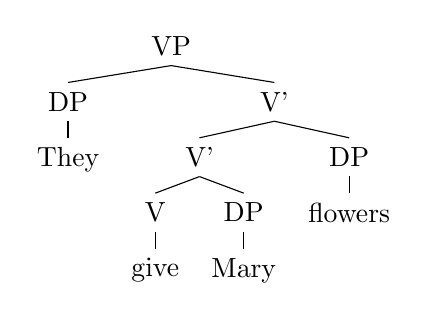
\begin{tikzpicture}
\tikzset{level distance=20pt, sibling distance=5pt}
\tikzset{every tree node/.style={align=center,anchor=north}}

\Tree[.{VP} [.{DP} They ] [.{V'} [.{V'} [.{V} give ] [.{DP} Mary ] ] [.{DP} flowers ] ] ] 

\end{tikzpicture}}

\begin{itemize}
\item RECEPIENT is higher than PATIENT.
\end{itemize}

\end{frame}

\begin{frame}[t,plain]{Argument from passive}

\ex.
\a. Mary is given flowers.
\b. *Flowers are given Mary.

\vspace{20pt}
\hspace{60pt}
\adjustbox{valign=t}{
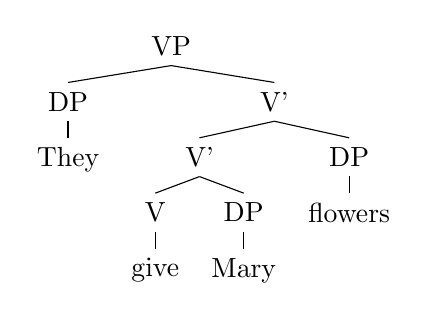
\begin{tikzpicture}
\tikzset{level distance=20pt, sibling distance=5pt}
\tikzset{every tree node/.style={align=center,anchor=north}}

\Tree[.{VP} [.{DP} They ] [.{V'} [.{V'} [.{V} give ] [.{DP} Mary ] ] [.{DP} flowers ] ] ] 

\end{tikzpicture}}

\end{frame}

\begin{frame}[t,plain]{}

\vspace{50pt}
\hspace{50pt}
\adjustbox{valign=t}{
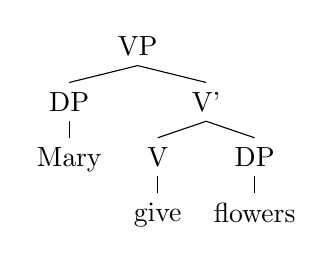
\begin{tikzpicture}
\tikzset{level distance=20pt, sibling distance=5pt}
\tikzset{every tree node/.style={align=center,anchor=north}}

\Tree[.{VP} [.{DP} Mary ] [.{V'} [.{V} give ] [.{DP} flowers ] ] ] 

\end{tikzpicture}}
\end{frame}


\begin{frame}[t,plain]{}

\vspace{50pt}
\hspace{50pt}
\adjustbox{valign=t}{
\begin{tikzpicture}
\tikzset{level distance=20pt, sibling distance=5pt}
\tikzset{every tree node/.style={align=center,anchor=north}}


\Tree[.{$\nu$P} [.{DP} They ] [.{$\nu'$} [.{$\nu$} [.{V} give\\{\setavm{\[V\]}} ] [.{$\nu$} $\emptyset$\\{\setavm{\[\textup{u}V, $\nu$\]}} ] ] [.{VP} [.{DP} Mary\\{\setavm{\[\textup{u}$\nu$\]}} ] [.{V'} [.{V} <give>\\{\setavm{\[V\]}} ] [.{DP} flowers\\{\setavm{\[\textup{u}$\nu$\]}} ] ] ] ] ] 


\end{tikzpicture}}

\end{frame}

\begin{frame}[t,plain]{Consequences: Burzio's Generalization}

\begin{itemize}
\item Active/Passive
\ex. 
\a. She observed him.
\b. He was observed.

\item Ergative alternation

\ex. \a. Harry boiled the water.
\b. The water boils.

\ex. \a. The enemy sank our boat.
\b. Our boat sank.

\ex. \a. Kirsten closed the door.
\b. The door closed.

\end{itemize}
\end{frame}

\begin{frame}[t,plain]{Active/Passive}



\vspace{20pt}
\hspace{20pt}
\parbox[t]{0.4\textwidth}{
Active construction

\bigskip
\bigskip

\adjustbox{valign=t}{
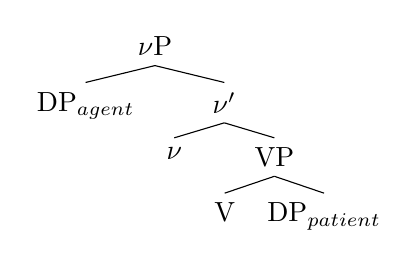
\begin{tikzpicture}
\tikzset{level distance=20pt, sibling distance=5pt}
\tikzset{every tree node/.style={align=center,anchor=north}}

\Tree[.{$\nu$P} [.{DP$_{agent}$} ] [.{$\nu'$} [.{$\nu$} ] [.{VP} [.{V} ] [.{DP$_{patient}$} ] ] ] ] 

\end{tikzpicture}}
}
\parbox[t]{0.4\textwidth}{
Passive construction

\bigskip
\bigskip

\adjustbox{valign=b}{
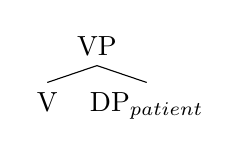
\begin{tikzpicture}
\tikzset{level distance=20pt, sibling distance=5pt}
\tikzset{every tree node/.style={align=center,anchor=north}}

\Tree[.{VP} [.{V} ] [.{DP$_{patient}$} ] ] 


\end{tikzpicture}}
}

\end{frame}

\begin{frame}[t,plain]{Ergative alternation}


\vspace{20pt}
\hspace{20pt}
\parbox[t]{0.5\textwidth}{
Harry boiled the water.

\bigskip
\bigskip

\adjustbox{valign=t}{
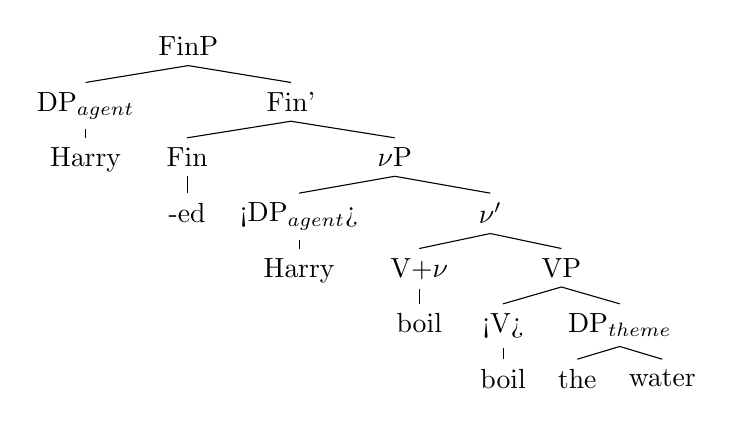
\begin{tikzpicture}
\tikzset{level distance=20pt, sibling distance=5pt}
\tikzset{every tree node/.style={align=center,anchor=north}}


\Tree[.{FinP} [.{DP$_{agent}$} Harry ] [.{Fin'} [.{Fin} -ed ] [.{$\nu$P} [.{<DP$_{agent}$>} Harry ] [.{$\nu'$} [.{V+$\nu$} boil ] [.{VP} [.{<V>} boil ] [.{DP$_{theme}$} the water ] ] ] ] ] ] 

\end{tikzpicture}}
}
\parbox[t]{0.4\textwidth}{
The water boils.

\bigskip
\bigskip

\adjustbox{valign=b}{
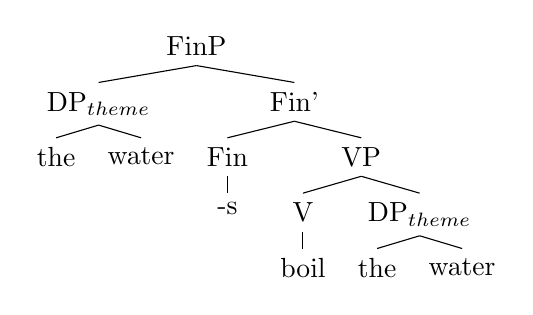
\begin{tikzpicture}
\tikzset{level distance=20pt, sibling distance=5pt}
\tikzset{every tree node/.style={align=center,anchor=north}}

\Tree[.{FinP} [.{DP$_{theme}$} the water ] [.{Fin'} [.{Fin} -s ] [.{VP} [.{V} boil ] [.{DP$_{theme}$} the water ] ] ] ] 

\end{tikzpicture}}
}
\end{frame}

\begin{frame}[t,plain]{}


\end{frame}

\end{document}
